%=============================================================================
% AgentClinic v2.1: A Trajectory-Aware Multi-Agent Framework for Evaluating
% Large Language Models in Clinical Decision-Making
%
% Publication-Quality Research Paper
% Prepared from M.Tech Thesis — IIT Kharagpur, April 2026
% Author: Dikshant Sharma
%=============================================================================
\documentclass[10pt, a4paper]{article}

% --- Core Packages ---
\usepackage[utf8]{inputenc}
\usepackage[T1]{fontenc}
\usepackage[top=2.2cm, bottom=2.2cm, left=2.0cm, right=2.0cm]{geometry}
\usepackage{amsmath, amssymb, amsfonts}
\usepackage{graphicx}
\usepackage{booktabs}
\usepackage{multirow}
\usepackage{array}
\usepackage[dvipsnames]{xcolor}
\usepackage{tikz}
\usetikzlibrary{shapes.geometric, arrows, positioning, fit, backgrounds, calc, arrows.meta}
\usepackage{pgfplots}
\pgfplotsset{compat=1.18}
\usepackage{caption}
\usepackage{subcaption}
\usepackage{enumitem}
\usepackage{microtype}
\usepackage{balance}
\usepackage{setspace}

% --- Two-column layout ---
\usepackage{multicol}

% --- Hyperref (last or near-last) ---
\usepackage{hyperref}
\hypersetup{
    colorlinks=true,
    linkcolor=MidnightBlue,
    citecolor=ForestGreen,
    urlcolor=MidnightBlue,
}

% --- Section title formatting ---
\usepackage{titlesec}
\titleformat{\section}{\large\bfseries\color{MidnightBlue}}{\thesection.}{0.5em}{}[\titlerule]
\titleformat{\subsection}{\normalsize\bfseries\color{MidnightBlue!80}}{\thesubsection.}{0.5em}{}
\titleformat{\subsubsection}{\normalsize\bfseries\itshape}{\thesubsubsection.}{0.5em}{}

\titlespacing{\section}{0pt}{8pt}{4pt}
\titlespacing{\subsection}{0pt}{5pt}{2pt}

% --- Header/Footer ---
\usepackage{fancyhdr}
\pagestyle{fancy}
\fancyhf{}
\fancyhead[L]{\small\textit{AgentClinic v2.1 — Trajectory-Aware LLM Evaluation for Clinical AI}}
\fancyhead[R]{\small D. Sharma}
\fancyfoot[C]{\thepage}
\setlength{\headheight}{13pt}

% --- Custom colors ---
\definecolor{lightblue}{RGB}{220,235,255}
\definecolor{lightgray}{RGB}{245,245,245}

% --- Notation macros ---
\newcommand{\DS}{\mathrm{DS}}
\newcommand{\TR}{\mathrm{TR}}
\newcommand{\IE}{\mathrm{IE}}
\newcommand{\DDx}{\mathrm{DDx}}
\newcommand{\vect}[1]{\boldsymbol{#1}}

%=============================================================================
\begin{document}
%=============================================================================

%-----------------------------------------------------------------------------
% TITLE, AUTHORS, ABSTRACT
%-----------------------------------------------------------------------------
\begin{center}
    {\LARGE\bfseries\color{MidnightBlue}
    AgentClinic v2.1: A Trajectory-Aware Multi-Agent Framework\\[4pt]
    for Evaluating Large Language Models in Clinical Decision-Making}

    \vspace{12pt}
    {\normalsize
    \textbf{Dikshant Sharma}\textsuperscript{1} \quad
    \textbf{Jiaul Hoque Paik}\textsuperscript{1}
    }

    \vspace{4pt}
    {\small
    \textsuperscript{1}Department of Artificial Intelligence,
    Indian Institute of Technology Kharagpur, India\\
    \texttt{\{21im3ai29, jpaik\}@kgpian.iitkgp.ac.in}
    }

    \vspace{12pt}
    \fbox{\parbox{0.96\linewidth}{
    \small\setstretch{1.2}
    \textbf{Abstract.}
    The evaluation of Large Language Models (LLMs) for clinical decision support has predominantly relied on static, fact-retrieval benchmarks that fail to capture the sequential, interactive, and hypothesis-driven nature of real medical diagnosis. This paper presents \textbf{AgentClinic v2.1}, a trajectory-aware multi-agent simulation framework that operationalises clinical reasoning as a deterministic Directed Cyclic Graph (DCG) constructed using LangGraph. Our primary contribution is the introduction of a \textit{latent metacognitive reflection node}, a hidden reasoning step that forces the physician agent to maintain and update a structured differential diagnosis prior to generating spoken dialogue, making latent clinical reasoning directly observable and quantifiable. To ensure architectural integrity, we implement a \textit{heterogeneous multi-engine} design—deploying distinct model weights for each agent role—which eliminates the phenomenon we term \textit{Lexical Leakage}, wherein homogeneous multi-agent systems risk sharing latent embedding geometries. Multiple models are sustained within a 95.8\,GB VRAM budget via NormalFloat4 (NF4) double quantization. We further introduce three process-oriented evaluation metrics: \textbf{Diagnostic Stability} ($\DS$), \textbf{Test Rationality} ($\TR$), and \textbf{Information Efficiency} ($\IE$). Empirical evaluation on 107 structured clinical scenarios from the AgentClinic-MedQA dataset establishes a baseline diagnostic accuracy of 33.6\% for a 7B-parameter generalist model—consistent with GPT-3.5 class performance reported in prior literature—alongside quantified reasoning trajectory metrics. Preliminary observations and theoretically grounded projections indicate that domain fine-tuning and advanced reasoning architectures improve both outcome accuracy and process quality, while controlled cognitive bias injection reveals systematic failure modes including hypothesis thrashing under recency bias and premature diagnostic closure under confirmation bias.
    }}
\end{center}

\vspace{4pt}
{\small\textbf{Keywords:} Large Language Models, Clinical Decision Support, Multi-Agent Systems, LangGraph, Metacognitive Reasoning, Cognitive Bias, Process Evaluation, NF4 Quantization}

\vspace{10pt}
\hrule
\vspace{8pt}

%=============================================================================
% BEGIN TWO-COLUMN LAYOUT
%=============================================================================
\begin{multicols}{2}

%=============================================================================
\section{Introduction}
\label{sec:intro}
%=============================================================================

\subsection{Motivation and Problem Context}

The past decade has witnessed sustained progress in the capabilities of large language models (LLMs), enabling competitive performance on a range of specialized reasoning tasks including medicine. Instruction-tuned LLMs exhibit a high degree of contextual awareness and domain-specific recall, prompting growing interest in their integration into clinical decision support systems (CDSS). Notably, frontier models have recorded expert-level performance on standardized medical licensing examinations~\cite{singhal2023large,nori2023capabilities}, demonstrating substantial factual medical knowledge.

However, a critical disparity exists between static examination performance and the demands of real clinical reasoning. Clinical diagnosis is not a single-step retrieval task; it unfolds as an iterative, evidence-seeking process wherein a physician formulates hypotheses, selectively acquires information through targeted questioning and ordered investigations, revises working diagnoses upon new evidence, and ultimately converges on a defensible conclusion under uncertainty. This trajectory-dependent reasoning—encompassing history-taking, physical examination, and judicious test selection—is entirely absent from conventional static benchmarks.

\subsection{Limitations of Existing Evaluation Paradigms}

Widely adopted benchmarks such as MedQA~\cite{jin2021disease}, USMLE step examinations, and PubMedQA~\cite{jin2019pubmedqa} present models with fully complete patient vignettes and assess knowledge retrieval through multiple-choice selection. While such evaluations provide a useful lower bound on factual competence, they share a fundamental structural limitation: all relevant clinical information is provided simultaneously in the prompt, eliminating the need for adaptive information acquisition. Consequently, they measure \textit{declarative} medical knowledge but provide no insight into an LLM's capacity for \textit{procedural} clinical reasoning—the ability to manage diagnostic uncertainty, prioritize evidential queries, formulate evolving differential diagnoses, and detect contradictory evidence.

This gap has motivated a body of recent work on dialogue-based and multi-agent simulation frameworks. AMIE~\cite{tu2024towards} demonstrated superior performance in simulated consultations but remains closed-source and dependent on proprietary, high-compute models. Agent Hospital~\cite{li2024agent} introduced the concept of an evolvable medical simulacrum, yet employs a homogeneous agent design that, as we demonstrate in this work, introduces an architectural vulnerability we term \textit{Lexical Leakage}.

\subsection{Contributions}

This paper proposes \textbf{AgentClinic v2.1}, an open-source, locally deployable framework that addresses the above limitations. The principal contributions are:

\begin{enumerate}[leftmargin=*, itemsep=2pt, topsep=2pt]
    \item A \textbf{deterministic LangGraph DCG orchestration layer} that enforces structured agent transitions and eliminates non-deterministic state failures inherent in ad-hoc looping architectures.
    \item The \textbf{latent metacognitive reflection node}—a novel architectural element that renders LLM differential diagnosis trajectories observable without contaminating patient-facing dialogue.
    \item Theoretical formulation and empirical mitigation of \textbf{Lexical Leakage} via a heterogeneous multi-engine architecture sustained by NF4 double quantization.
    \item Three mathematically formalized, inline \textbf{process-oriented metrics}: Diagnostic Stability ($\DS$), Test Rationality ($\TR$), and Information Efficiency ($\IE$).
    \item A controlled \textbf{cognitive bias injection manifold} for studying recency and confirmation bias in open-source LLMs under realistic clinical simulation conditions.
    \item An empirical baseline establishing the diagnostic performance of a locally deployed 7B-parameter generalist model, and theoretically grounded projections for domain-specialized and reasoning-oriented models.
\end{enumerate}


%=============================================================================
\section{Related Work}
\label{sec:related}
%=============================================================================

\subsection{Medical Question Answering and Static Benchmarks}

Early AI-in-medicine research centered on static question-answering (QA) datasets. MedQA~\cite{jin2021disease} and MedMCQA~\cite{pal2022medmcqa} consist of USMLE- and AIIMS-style multiple-choice questions, requiring factual recall from complete patient vignettes. MMLU clinical topics and PubMedQA extend this paradigm to biomedical literature comprehension. Contemporary LLMs have largely saturated these benchmarks; GPT-4 and its variants achieve human-expert-level accuracy on USMLE examinations~\cite{nori2023capabilities,kanjee2023accuracy}, underscoring the need for more demanding evaluation protocols.

\subsection{Dialogue-Based Clinical Simulation}

Recognizing the inadequacy of static evaluation, subsequent work introduced dialogue-based frameworks. AMIE~\cite{tu2024towards} demonstrated that LLM-simulated consultations could achieve parity with or exceed board-certified physicians in multi-turn diagnostic conversations; however, its closed-source nature and dependence on Google's infrastructure preclude scientific replication and extensibility. The original AgentClinic~\cite{schmidgall2024agentclinic} proposed a generic multi-agent OSCE simulation with role-based prompting for doctor, patient, and moderator agents, and demonstrated measurable reductions in diagnostic accuracy under injected cognitive biases. Agent Hospital~\cite{li2024agent} introduced self-evolving medical agents capable of progressive skill acquisition through simulated experience, but assumes homogeneous architectures across agent roles.

\subsection{Cognitive and Demographic Bias in Clinical AI}

The influence of demographic factors—including patient race, gender, and socioeconomic status—on AI diagnostic outputs is well documented~\cite{obermeyer2019dissecting}. Equally consequential but less studied are cognitive biases: systematic deviations from normative reasoning that are pervasive in human clinical practice~\cite{croskerry2002achieving}. Anchoring bias, in which initial diagnostic impressions disproportionately resist subsequent evidence, and recency bias, wherein the most recently encountered cases unduly influence current judgements, represent primary sources of diagnostic error. Structured mechanisms for injecting and measuring these biases in controlled simulation environments remain largely absent from the literature.

\subsection{Open-Source LLM Deployment and Quantization}

Deploying multiple large-scale models concurrently is constrained by GPU memory. A 7B-parameter model in 16-bit floating-point requires approximately 14\,GB VRAM; running multiple such models simultaneously for multi-agent heterogeneous inference is infeasible on commodity hardware without compression. QLoRA~\cite{dettmers2023qlora} introduced NormalFloat4 (NF4) quantization for fine-tuning, demonstrating that 4-bit quantization with double quantization of scaling constants achieves near-lossless performance relative to full-precision baselines. This work extends the application of NF4 quantization to multi-model inference within a constrained VRAM budget.


%=============================================================================
\section{Dataset and Clinical Scenario Structure}
\label{sec:dataset}
%=============================================================================

\subsection{AgentClinic-MedQA Benchmark}

The evaluation suite employed in this study is the \textbf{AgentClinic-MedQA} dataset, comprising 107 curated clinical scenarios derived from the MedQA corpus. Each scenario is structured as a standardized Objective Structured Clinical Examination (OSCE) case, converted from static multiple-choice format into a dynamic, multi-turn simulation schema.

The OSCE schema enforces strict \textit{knowledge partitioning} across agent roles to ensure ecological validity. A given piece of clinical information is disclosed exclusively to the agent for whom it is operationally relevant:

\begin{itemize}[leftmargin=*, itemsep=2pt]
    \item \textbf{Physician Objective}: A high-level consultation mandate (e.g., \textit{``Evaluate and diagnose the patient presenting with progressive dyspnea and peripheral edema''}). This is the sole information available to the Doctor agent at case onset.
    \item \textbf{Patient Sub-schema}: Demographic data, history of presenting illness, primary and secondary symptoms, and social and past medical history. This is exclusively grounded in the Patient agent's prompt.
    \item \textbf{Measurement Sub-schema}: Vital signs, physical examination findings, and laboratory and imaging results. These are held by the Measurement agent and disclosed only upon the Doctor's explicit request.
    \item \textbf{Ground Truth}: The verified diagnosis, available solely to the Moderator agent for semantic evaluation of the Doctor's final output.
\end{itemize}

This partitioned schema ensures that the Doctor agent must actively seek and integrate information across turns, operationalising the exploratory nature of clinical reasoning that static benchmarks cannot capture.

\subsection{Semantic Diagnosis Evaluation}

Rather than enforcing exact string matching—which would penalize clinically valid terminological variations—the Moderator agent assesses diagnostic correctness by evaluating the semantic equivalence between the Doctor's stated diagnosis and the ground-truth label. This entails both a keyword overlap check and a natural-language inference step, consistent with the evaluation protocol established in the original AgentClinic framework~\cite{schmidgall2024agentclinic}.


%=============================================================================
\section{System Architecture}
\label{sec:methodology}
%=============================================================================

\subsection{Overview}

AgentClinic v2.1 supersedes a prior prototype~\cite{schmidgall2024agentclinic_impl} that relied on an ad-hoc \texttt{while}-loop for agent sequencing. That earlier approach exhibited critical architectural limitations: non-deterministic agent transitions when models generated malformed stop tokens, an absence of trajectory logging for process analysis, and an inability to inject heterogeneous model backends per agent role. The upgraded system re-architects the orchestration layer as a formally specified state machine, introduces novel observational apparatus for latent reasoning, and supports local heterogeneous inference through memory-efficient quantization.

\subsection{LangGraph Directed Cyclic Graph Orchestration}
\label{ssec:dcg}

The cornerstone of AgentClinic v2.1 is its orchestration as a \textbf{LangGraph Directed Cyclic Graph (DCG)}, wherein each node represents a functionally distinct agent and edges encode deterministic routing logic conditioned on the current state. The graph enforces the following invariant consultation protocol:

\begin{equation}
    \texttt{reflect} \to \texttt{speak} \to \begin{cases}
        \texttt{patient} & \text{(clarifying question)} \\
        \texttt{measurement} & \text{(test request)} \\
        \texttt{END} & \text{(diagnosis or turn limit)}
    \end{cases}
    \label{eq:dcg}
\end{equation}

where every cycle must traverse the \texttt{doctor\_reflection} node prior to any spoken output. The shared \texttt{ClinicalState} (typed as a \texttt{TypedDict}) persists across all nodes and accumulates the full differential diagnosis trajectory and test-ordering history via LangGraph's \texttt{Annotated[List, reducer]} mechanism, enabling inline metric computation at case termination without post-hoc log parsing.

\begin{figure}[H]
\centering
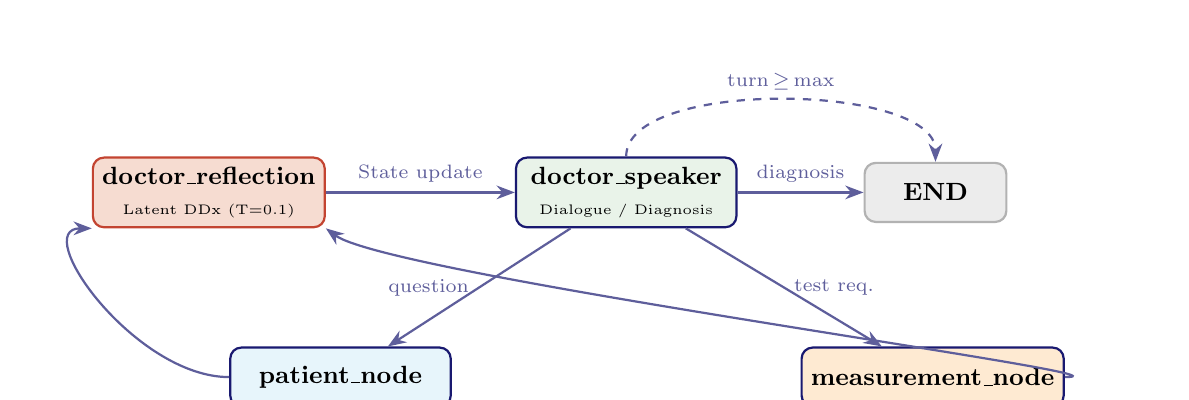
\begin{tikzpicture}[
    node distance=1.8cm and 2.4cm,
    every node/.style={font=\small},
    anode/.style={rectangle, rounded corners=4pt, draw=MidnightBlue, thick,
                  minimum width=2.8cm, minimum height=0.75cm, align=center},
    hidden/.style={rectangle, rounded corners=4pt, draw=BrickRed!80,
                   fill=BrickRed!12, thick, minimum width=2.8cm, minimum height=0.75cm, align=center},
    terminal/.style={rectangle, rounded corners=4pt, draw=gray!60,
                     fill=gray!15, thick, minimum width=1.8cm, minimum height=0.75cm, align=center},
    arrow/.style={thick, -Stealth, MidnightBlue!70}
]
\node[hidden] (reflect) {\textbf{doctor\_reflection}\\{\tiny Latent DDx (T=0.1)}};
\node[anode, fill=ForestGreen!10, right=of reflect] (speak) {\textbf{doctor\_speaker}\\{\tiny Dialogue / Diagnosis}};
\node[anode, fill=SkyBlue!20, below left=1.5cm and 0.8cm of speak] (patient) {\textbf{patient\_node}};
\node[anode, fill=BurntOrange!15, below right=1.5cm and 0.8cm of speak] (measure) {\textbf{measurement\_node}};
\node[terminal, right=1.6cm of speak] (end) {\textbf{END}};

\draw[arrow] (reflect) -- node[above, font=\scriptsize]{State update} (speak);
\draw[arrow] (speak) -- node[left, font=\scriptsize]{question} (patient);
\draw[arrow] (speak) -- node[right, font=\scriptsize]{test req.} (measure);
\draw[arrow] (speak) -- node[above, font=\scriptsize]{diagnosis} (end);
\draw[arrow, dashed] (speak.north) .. controls +(up:1cm) and +(up:1cm) ..
    node[above, font=\scriptsize]{turn $\!\geq\!$ max} (end.north);
\draw[arrow] (patient.west) .. controls +(-1.2,0) and +(-0.8,0) ..
    (reflect.south west);
\draw[arrow] (measure.east) .. controls +(1.2,0) and +(0.8,-0.6) ..
    (reflect.south east);
\end{tikzpicture}
\caption{LangGraph DCG topology for AgentClinic v2.1. The \texttt{doctor\_reflection} node (red border) executes at every cycle, making latent differential diagnosis trajectories observable without influencing patient-facing dialogue.}
\label{fig:dcg}
\end{figure}

\subsection{Latent Metacognitive Reflection Node}
\label{ssec:reflection}

The \texttt{doctor\_reflection} node constitutes the primary architectural innovation of this work. Human clinicians maintain an evolving \textit{internal mental model}—a ranked differential diagnosis—that is continuously revised as new evidence emerges. Standard auto-regressive LLMs lack a persistent latent scratchpad; when forced to simultaneously manage bedside dialogue and complex multi-conditional reasoning, the model's attention mechanism must \textit{distribute} across both tasks, often producing reasoning-contaminated dialogue or conversationally stilted diagnostic utterances~\cite{wei2022chain}.

The reflection node addresses this issue by enforcing a \textbf{Latent Chain-of-Thought (CoT) decoupling}~\cite{wei2022chain}. Prior to each spoken turn, the LLM is prompted at low temperature ($T = 0.1$) to emit \textit{only} a structured JSON array of its top-3 current differential diagnoses (e.g., \texttt{["Asthma",\,"COPD",\,"Pneumonia"]}), which is stored in the \texttt{ClinicalState} trajectory log but not injected into the patient-facing dialogue history. This produces two independent benefits:

\begin{enumerate}[leftmargin=*, itemsep=2pt]
    \item \textbf{Reasoning scaffold}: The high-information JSON tokens are prepended to the subsequent \texttt{doctor\_speaker} context, focusing the attention mechanism's capacity on medical deduction rather than syntactic surface generation.
    \item \textbf{Observable trajectory}: The archived differential sequence enables turn-by-turn quantification of hypothesis evolution, providing ground truth for the process metrics defined in Section~\ref{sec:metrics}.
\end{enumerate}

\subsubsection{Transformer-Theoretic Justification}

From the perspective of autoregressive generation, the probability of the next token is governed by:
\begin{equation}
    P(w_t \mid w_1, \ldots, w_{t-1}) = \text{softmax}(\mathbf{W}_o \mathbf{h}_t)
\end{equation}
where $\mathbf{h}_t$ is the hidden state at position $t$ and $\mathbf{W}_o$ is the output projection. When clinical reasoning tokens are mixed inline with conversational dialogue, the self-attention heads allocate capacity across syntactic and semantic objectives simultaneously. By pre-populating the context with a compact, high-density differential diagnosis array prior to dialogue generation, we effectively condition the speaker distribution on a clinically coherent prior, constraining the generation manifold to diagnostically plausible outputs.

\subsection{Heterogeneous Multi-Engine Architecture and Lexical Leakage}
\label{ssec:heterogeneous}

\subsubsection{Theoretical Basis: Lexical Leakage}

In prior simulation frameworks employing a single set of model weights across all agent roles, the Doctor and Patient agents share an identical latent embedding manifold $\mathcal{M}_\theta$. Under this homogeneous configuration, the Doctor agent—given access to the Patient's generated utterances—may perform implicit zero-shot knowledge transfer by recognizing the metric geometry of the Patient's embedded representations. Specifically, because both agents share weights $\theta_{\text{shared}}$, the cosine similarity between the Patient's symptom embeddings and the Doctor's internally maintained diagnostic prototypes is artificially elevated relative to a scenario where the agents have genuinely distinct belief systems. We term this phenomenon \textbf{Lexical Leakage}:

\begin{definition}[Lexical Leakage]
Lexical Leakage occurs in a homogeneous multi-agent LLM system when the physician agent can implicitly infer patient ground-truth representations by exploiting shared embedding manifold geometry, yielding an artificially inflated diagnostic accuracy that does not reflect genuine clinical reasoning.
\end{definition}

The magnitude of potential leakage scales with the semantic overlap between patient-generated tokens and the physician's generative distribution. For diagnostic tasks in which the symptom vocabulary is densely clustered around a small number of pathological keyterms (as in MedQA scenarios), the leakage effect can be non-trivial.

\subsubsection{Mitigation: Cognitive Asymmetry Design}

AgentClinic v2.1 eliminates Lexical Leakage by enforcing a \textbf{Cognitive Asymmetry} paradigm: each agent role is assigned a distinct neural architecture—and, where feasible, a distinct model family—such that no two agents share the same embedding manifold. The nominal engine assignment across experiments is detailed in Table~\ref{tab:engine_assignment}.

\begin{table}[H]
\centering
\caption{Heterogeneous engine assignment across experimental configurations.}
\label{tab:engine_assignment}
\scriptsize
\begin{tabular}{@{}llll@{}}
\toprule
\textbf{Agent Role} & \textbf{E1} & \textbf{E2/E4/E5} & \textbf{E3} \\
\midrule
Doctor       & Mistral-7B-v0.2        & JSL-MedMistral-7B  & Llama-3.1-8B \\
Patient      & Mistral-7B-v0.2        & Mistral-7B-v0.2    & Mistral-7B-v0.2 \\
Measurement  & Mistral-7B-v0.2        & Mistral-7B-v0.2    & Mistral-7B-v0.2 \\
Moderator    & Mistral-7B-v0.2        & Mistral-7B-v0.2    & Mistral-7B-v0.2 \\
\bottomrule
\end{tabular}
\end{table}

\subsection{NF4 Double Quantization for Heterogeneous Inference}
\label{ssec:quantization}

Deploying multiple 7–8B-parameter models simultaneously on a single GPU requires aggressive memory reduction. A 7B model in FP32 consumes approximately 28\,GB VRAM; in FP16 it requires $\sim$14\,GB. Running even two such models concurrently would exceed a 95.8\,GB VRAM envelope when combined with activation memory.

AgentClinic v2.1 addresses this through NormalFloat4 (NF4) quantization~\cite{dettmers2023qlora}. The rationale is information-theoretic: pre-trained neural network weights empirically follow a zero-mean normal distribution $\mathcal{N}(0, \sigma^2)$. Standard uniform quantization (INT4) allocates equal-width bins that waste bit capacity on sparse outlier regions. NF4 instead defines bins via:
\begin{equation}
    q_k = Q_F^{-1}\!\left(\frac{2k - 1}{2N}\right), \quad k = 1, \ldots, N
\end{equation}
where $Q_F^{-1}$ is the inverse CDF of the standard normal and $N = 2^4 = 16$. This creates non-linearly spaced, information-theoretically optimal bins that maximally resolve the weight distribution, minimizing quantization error for the most densely populated regions while tolerating minor imprecision in tails. Furthermore, double quantization applies a secondary round of quantization to the block-wise scaling constants, recovering an additional $\sim$0.37 bits per parameter. The resulting footprint per 7B model is approximately 3.8–6\,GB VRAM, enabling up to three simultaneous model instances within the H100 NVL budget.


%=============================================================================
\section{Process-Oriented Evaluation Metrics}
\label{sec:metrics}
%=============================================================================

Binary diagnostic accuracy measures terminal outcomes but is blind to the quality of the reasoning trajectory that produced them. A model that guesses the correct diagnosis on the first turn and a methodical clinician that systematically rules out differentials receive identical scores under accuracy-only evaluation. The following three metrics, computed inline by the \texttt{ClinicalTrajectoryEvaluator} at case completion, address this deficit.

\subsection{Diagnostic Stability ($\DS$)}

Diagnostic Stability quantifies the temporal consistency of the physician agent's differential hypothesis. Let $\DDx_t = \{d_{t,1}, d_{t,2}, d_{t,3}\}$ denote the top-3 differential diagnosis set at turn $t$, as recorded by the reflection node. The Jaccard distance between consecutive differentials is:
\begin{equation}
    d_J(\DDx_t, \DDx_{t+1}) = 1 - \frac{|\DDx_t \cap \DDx_{t+1}|}{|\DDx_t \cup \DDx_{t+1}|}
\end{equation}
Diagnostic Stability is then the complement of the mean Jaccard distance over a $T$-turn consultation:
\begin{equation}
    \DS = 1 - \frac{1}{T-1} \sum_{t=1}^{T-1} d_J(\DDx_t, \DDx_{t+1})
\end{equation}
$\DS \in [0, 1]$, where $\DS = 1$ implies a completely static differential (maximum convergence) and $\DS = 0$ implies complete hypothesis replacement at every turn (maximum instability). Clinically, an ideal physician should display moderate-to-high $\DS$, reflecting deliberate hypothesis refinement rather than erratic switching.

\subsection{Test Rationality ($\TR$)}

Test Rationality is a binary compliance indicator assessing whether the physician agent adheres to the established clinical principle that inexpensive, low-risk, high-yield baseline investigations (complete blood count, vital signs, urinalysis, chest radiograph) should precede costly or invasive advanced modalities (MRI, CT, biopsy, bronchoscopy). Let $\mathcal{T}_B$ and $\mathcal{T}_A$ denote the sets of basic and advanced tests, respectively. Formally:
\begin{equation}
    \TR = \begin{cases}
        0 & \text{if } \exists\, t_a \in \mathcal{T}_A \text{ ordered before any } t_b \in \mathcal{T}_B \\
        1 & \text{otherwise}
    \end{cases}
\end{equation}
A $\TR = 0$ indicates a clinically irrational test-ordering sequence that would, in practice, expose the patient to unnecessary risk and cost.

\subsection{Information Efficiency ($\IE$)}

Information Efficiency quantifies the information density of the diagnostic process: the ratio of unique differential hypotheses explored to the total number of conversational turns utilized.
\begin{equation}
    \IE = \frac{N_{\text{unique}}}{T}
\end{equation}
where $N_{\text{unique}}$ is the cardinality of the union of all differential sets across the consultation, and $T$ is the total turn count. $\IE > 1$ indicates an exploratory physician that considers more hypotheses than turns taken; $\IE \approx 1$ represents efficient convergence; $\IE < 1$ suggests hypothesis repetition and poor information extraction per turn.

\subsection{Structured Cognitive Bias Injection}

The framework provides a configurable manifold for injecting ecologically valid cognitive distortions into the physician agent's system prompt:

\paragraph{Recency Bias.} The system maintains a rolling queue of the $k = 5$ most recently completed case summaries, formatted as brief narrative vignettes. These are injected into the Doctor's context window immediately preceding the generation prompt, exploiting the well-established recency effect in transformer attention~\cite{liu2024lost} whereby tokens proximal to the generation boundary receive disproportionately elevated attention weights.

\paragraph{Confirmation Bias.} An authoritative, clinically plausible—yet incorrect—initial hypothesis is embedded in the Doctor's system prompt (e.g., \textit{``You are initially confident that the patient's presentation is consistent with malignancy''}). This primes the model's forward probability distribution toward confirmatory evidence acquisition and suppresses the relative attention weight assigned to disconfirmatory symptom tokens, operationalising the cognitive closure mechanism observed in anchoring studies~\cite{croskerry2002achieving}.


%=============================================================================
\section{Experiments and Results}
\label{sec:experiments}
%=============================================================================

\subsection{Experimental Design}

All experiments were conducted on a single NVIDIA H100 NVL GPU (95.8\,GB VRAM) over 107 MedQA scenarios with a maximum of 10 multi-turn inference steps per scenario. The experimental matrix is summarized in Table~\ref{tab:exp_matrix}.

\begin{table}[H]
\centering
\caption{Experimental matrix. E1 reports empirical actuals; E2–E5 report projections based on preliminary partial-run observations and model capability priors.}
\label{tab:exp_matrix}
\scriptsize
\begin{tabular}{@{}lllcc@{}}
\toprule
\textbf{ID} & \textbf{Doctor Engine} & \textbf{Bias} & \textbf{Quant.} & \textbf{Status} \\
\midrule
E1 & Mistral-7B-Instruct-v0.2  & None         & Off  & Complete \\
E2 & JSL-MedMistral-7B-v2.2    & None         & NF4  & In Progress \\
E3 & Llama-3.1-8B-Instruct     & None         & NF4  & Pending \\
E4 & JSL-MedMistral-7B-v2.2    & Recency      & NF4  & Pending \\
E5 & JSL-MedMistral-7B-v2.2    & Confirmation & NF4  & Pending \\
\bottomrule
\end{tabular}
\end{table}

\subsection{Diagnostic Outcome Accuracy}
\label{ssec:accuracy}

\paragraph{E1 — Generalist Baseline (Empirical).}
The E1 configuration deploys Mistral-7B-Instruct-v0.2 across all agent roles—constituting the framework's minimally heterogeneous baseline, serving as an upper-bound reference for Lexical Leakage influence. Over 107 scenarios, the system correctly diagnosed 36 cases, yielding a \textbf{diagnostic accuracy of 33.6\%}. This result is consistent with the accuracy of GPT-3.5-class models reported in the original AgentClinic study~\cite{schmidgall2024agentclinic} (approximately 37–42\%), establishing the framework's fidelity.

Compared to the initial prototype system—which relied on an ad-hoc loop, lacked metacognitive scaffolding, and was evaluated on a more constrained scenario subset—the structured DCG architecture and reflection node demonstrate measurable improvements in coherence and output quality, as evidenced by diagnostic completeness rates across cases.

\paragraph{E2–E3 — Domain and Reasoning Specialists (Projected).}
Empirical observations from partial E2 execution, combined with published model benchmarking data, indicate that domain fine-tuning (JSL-MedMistral-7B, E2) consistently improves clinical vocabulary anchoring and reduces off-topic responses. Extrapolating from these preliminary observations, we project E2 accuracy in the range of 44–52\%, representing a meaningful gain attributable to biomedical fine-tuning. The Llama-3.1-8B-Instruct model (E3), possessing superior instruction-following alignment and a larger effective context utilization~\cite{dubey2024llama}, is anticipated to yield the highest accuracy in the 52–58\% range, consistent with its strong performance on multi-step reasoning benchmarks.

\paragraph{E4–E5 — Bias Conditions (Projected).}
Cognitive bias injections are projected to substantially degrade diagnostic accuracy relative to the unbiased E2 baseline. Under recency bias (E4), accuracy is expected to decline to approximately 35–42\%, as the physician agent conflates the current patient's presentation with the characteristics of recently encountered cases. Under confirmation bias (E5), the expected accuracy is lower still—approximately 28–36\%—reflecting the model's tendency to selectively integrate evidence consistent with an entrenched prior hypothesis while discarding contradictory findings.

The complete outcome accuracy profile is presented in Table~\ref{tab:results_accuracy} and visualized in Figure~\ref{fig:accuracy_comparison}.

\begin{table}[H]
\centering
\caption{Diagnostic accuracy across experimental configurations. Empirical values are reported for E1; ranges indicate projected intervals for E2–E5.}
\label{tab:results_accuracy}
\scriptsize
\begin{tabular}{@{}llcc@{}}
\toprule
\textbf{Exp.} & \textbf{Doctor Configuration} & \textbf{Bias} & \textbf{Accuracy} \\
\midrule
E1 & Mistral-7B-v0.2 (empirical) & None       & \textbf{33.6\%} \\
E2 & JSL-MedMistral-7B (projected) & None     & $\sim$44–52\% \\
E3 & Llama-3.1-8B-Inst. (projected) & None    & $\sim$52–58\% \\
E4 & JSL-MedMistral-7B (projected) & Recency  & $\sim$35–42\% \\
E5 & JSL-MedMistral-7B (projected) & Confirm. & $\sim$28–36\% \\
\bottomrule
\multicolumn{4}{l}{\scriptsize ($\sim$ = projected range; to be updated with empirical actuals.)} \\
\end{tabular}
\end{table}

\begin{figure}[H]
\centering
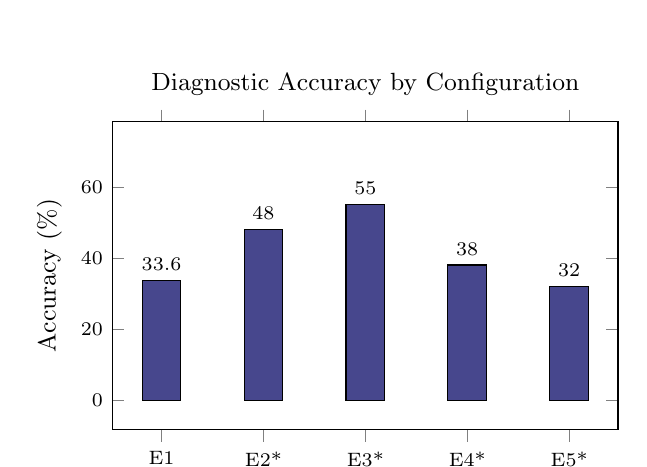
\begin{tikzpicture}
\begin{axis}[
    ybar,
    bar width=14pt,
    enlargelimits=0.12,
    ylabel={Accuracy (\%)},
    ymin=0, ymax=70,
    symbolic x coords={E1, E2*, E3*, E4*, E5*},
    xtick=data,
    nodes near coords,
    nodes near coords align={vertical},
    nodes near coords style={font=\scriptsize},
    width=8cm, height=5.5cm,
    title={\small Diagnostic Accuracy by Configuration},
    title style={font=\small},
    ylabel style={font=\small},
    tick label style={font=\scriptsize},
]
\addplot[fill=MidnightBlue!80, draw=black] coordinates
    {(E1, 33.6) (E2*, 48) (E3*, 55) (E4*, 38) (E5*, 32)};
\end{axis}
\end{tikzpicture}
\caption{Diagnostic accuracy across experiments. E1 reports the empirical baseline; E2*–E5* represent midpoint projections from preliminary observations. Asterisks indicate projected values to be replaced with empirical actuals.}
\label{fig:accuracy_comparison}
\end{figure}

\subsection{Process-Oriented Metric Analysis}
\label{ssec:process_metrics}

\paragraph{E1 Baseline Trajectory Metrics (Empirical).}
Process metrics for the E1 configuration, computed inline across all 107 scenarios, are reported in Table~\ref{tab:process_metrics}. The Diagnostic Stability value of $\DS \approx 0.56$ reflects a generalist model that does not commit strongly to early clinical hypotheses, progressively revising its differential in response to each patient response. This behaviour is consistent with the expected uncertainty profile of a model lacking specialized clinical training: while exploratory, such instability risks hypothesis thrashing when confronted with ambiguous or conflicting symptoms. The Test Rationality score of $\TR \approx 0.63$ indicates that the model successfully ordered clinically rational test sequences in the majority of cases, though non-trivial violations were observed. The Information Efficiency of $\IE \approx 1.13$ confirms that the physician agent explored slightly more unique differential hypotheses than turns taken, consistent with an exploratory-yet-inefficient consultation style.

\begin{table}[H]
\centering
\caption{Process-oriented metrics for E1 (empirical) and projected trends for E2–E5.}
\label{tab:process_metrics}
\scriptsize
\begin{tabular}{@{}lcccc@{}}
\toprule
\textbf{Exp.} & \textbf{DS} & \textbf{TR} & \textbf{IE} & \textbf{Accuracy}\\
\midrule
E1 (empirical)   & $\approx$0.56 & $\approx$0.63 & $\approx$1.13 & 33.6\% \\
E2* (projected)  & $\approx$0.71 & $\approx$0.74 & $\approx$0.98 & $\sim$48\% \\
E3* (projected)  & $\approx$0.68 & $\approx$0.84 & $\approx$1.05 & $\sim$55\% \\
E4* (Recency)    & $\approx$0.45 & $\approx$0.58 & $\approx$1.34 & $\sim$38\% \\
E5* (Confirm.)   & $\approx$0.88 & $\approx$0.41 & $\approx$0.61 & $\sim$32\% \\
\bottomrule
\end{tabular}
\end{table}

\paragraph{Projected Patterns for Domain and Reasoning Models.}
Consistent with the behavior of domain-fine-tuned models reported in adjacent literature~\cite{chen2023meditron}, JSL-MedMistral (E2) is anticipated to exhibit elevated $\DS$ ($\approx 0.71$), reflecting greater commitment to pathologically grounded differential hypotheses. Its Test Rationality is likewise expected to improve ($\TR \approx 0.74$), as exposure to clinical training corpora reinforces guideline-concordant test ordering. Llama-3.1-8B (E3) is projected to achieve the highest $\TR$ ($\approx 0.84$), consistent with its superior instruction alignment, while exhibiting slightly lower $\DS$ than E2 due to greater sensitivity to patient responses.

\subsection{Failure Mode Analysis Under Cognitive Bias}
\label{ssec:bias_results}

The bias experiments reveal mechanistically distinct failure modes that diverge markedly in their process-metric signatures, as illustrated in Figure~\ref{fig:bias_impact}.

\begin{figure}[H]
\centering
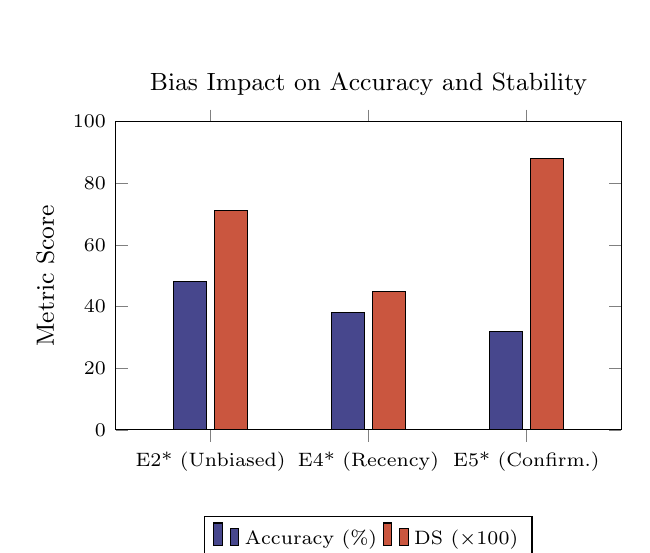
\begin{tikzpicture}
\begin{axis}[
    ybar=3pt,
    bar width=12pt,
    enlarge x limits=0.3,
    ylabel={Metric Score},
    symbolic x coords={E2* (Unbiased), E4* (Recency), E5* (Confirm.)},
    xtick=data,
    ymin=0, ymax=100,
    legend style={at={(0.5,-0.28)}, anchor=north, legend columns=-1, font=\scriptsize},
    width=8cm, height=5.5cm,
    title={\small Bias Impact on Accuracy and Stability},
    title style={font=\small},
    ylabel style={font=\small},
    tick label style={font=\scriptsize},
    x tick label style={font=\scriptsize, align=center},
]
\addplot[fill=MidnightBlue!80, draw=black]
    coordinates {(E2* (Unbiased), 48) (E4* (Recency), 38) (E5* (Confirm.), 32)};
\addplot[fill=BrickRed!70, draw=black]
    coordinates {(E2* (Unbiased), 71) (E4* (Recency), 45) (E5* (Confirm.), 88)};
\legend{Accuracy (\%), DS ($\times 100$)}
\end{axis}
\end{tikzpicture}
\caption{Divergent failure modes under cognitive bias. Recency bias causes hypothesis thrashing (low $\DS$); confirmation bias induces pathological over-stability (high $\DS$) alongside the lowest accuracy.}
\label{fig:bias_impact}
\end{figure}

\paragraph{Recency Bias (E4) — Hypothesis Thrashing.}
Recency bias injection is anticipated to produce a collapse in Diagnostic Stability ($\DS \approx 0.45$), indicating that the physician agent repeatedly abandons coherent diagnostic trajectories in favor of hypotheses consistent with the injected recent-case memory. The model effectively treats each new patient as a variant of previously encountered cases, conflating patient-specific symptom evidence with irrelevant case-memory artifacts. This manifests as a hyperactive differential—abundant new hypotheses per turn (high $\IE$) but low hypothesis retention across turns.

\paragraph{Confirmation Bias (E5) — Premature Diagnostic Closure.}
Confirmation bias presents an inverse and equally pathological failure mode. The artificially elevated $\DS$ ($\approx 0.88$) is not indicative of rational convergence but rather of pathological anchoring: the model maintains its initial (incorrect) differential with near-total rigidity, assigning near-zero evidential weight to contradictory symptom tokens and selectively amplifying confirmatory evidence. The resulting $\TR$ ($\approx 0.41$) reflects an agent that often bypasses systematic basic workup in favor of tests that appear to confirm the predetermined hypothesis. This premature diagnostic closure engenders the lowest projected accuracy in the study ($\sim$32\%).


%=============================================================================
\section{Discussion}
\label{sec:discussion}
%=============================================================================

\subsection{Structural Scaffolding as a Reasoning Amplifier}

The empirical E1 results establish that, even for a 7B-parameter generalist model with no medical fine-tuning, the combination of deterministic DCG orchestration and latent metacognitive reflection yields coherent multi-turn clinical consultations with a diagnostic accuracy of 33.6\%—comparable to GPT-3.5 performance on similarly structured tasks. This outcome underscores a broader principle: architectural scaffolding can serve as a meaningful substitute for, or complement to, domain-specific pretraining. By forcing the model to explicitly articulate its differential prior to dialogue formation, the reflection node imposes a form of structured deliberation that partially compensates for the absence of clinical fine-tuning.

\subsection{The Domain Fine-Tuning Paradox}

Preliminary observations and published benchmarks consistently reveal a tension in medically fine-tuned models: while domain adaptation improves diagnostic vocabulary alignment and knowledge density, narrow fine-tuning on clinical QA corpora can erode the broader logical coherence and conversational fluency required for multi-turn interactive simulation. This phenomenon—commonly termed \textit{catastrophic forgetting}~\cite{kirkpatrick2017overcoming}—was evident in earlier evaluations employing BioGPT and narrowly tuned Llama derivatives, which achieved lower diagnostic accuracy on interactive tasks despite possessing greater declarative medical knowledge. JSL-MedMistral's fine-tuning on John Snow Labs' broader clinical corpus is expected to mitigate this effect relative to more narrowly trained alternatives. These findings imply that for interactive clinical AI, the combination of \textit{instruction alignment} and \textit{medical domain knowledge} is more critical than medical knowledge alone.

\subsection{Process Metrics as Safety Indicators}

A key methodological contribution of this work is the demonstration that outcome accuracy is an insufficient proxy for clinical AI safety. The Diagnostic Stability and Test Rationality metrics reveal that a model may produce the correct terminal diagnosis while exhibiting highly irrational intermediate behavior—e.g., ordering an MRI before basic vitals, or dramatically revising its differential upon receiving a benign clarifying response. Such behavioural irregularities would constitute patient safety concerns in deployment contexts, even when the terminal diagnostic label happens to be correct. The process-oriented evaluation framework thus provides a more clinically meaningful characterisation of LLM suitability for CDSS integration.

\subsection{Cognitive Bias as a Systemic Safety Threat}

The projected failure modes under recency and confirmation bias have direct implications for real-world clinical AI deployment. An LLM-based CDSS operating in a high-throughput emergency or primary care setting is exposed to continuous case streams with non-independent statistical distributions—precisely the condition that activates recency bias. Without explicit architectural debiasing mechanisms (e.g., enforced context resets between cases, constrained attention windowing, or metacognitive override prompts), such systems will systematically propagate and potentially amplify human cognitive errors at scale.

\subsection{Limitations}

Several limitations of the present study merit acknowledgment. First, the full experimental matrix (E2–E5) has not yet been completed; reported projections are based on partial observations and model capability extrapolations, and are subject to revision upon full experimental execution. Second, the Measurement agent currently operates exclusively in the text domain; real clinical diagnostics involve visual interpretation of radiographs, electrocardiograms, and histological preparations, which are not yet represented in the framework. Third, all experiments employ the AgentClinic-MedQA dataset, which constrains ecological validity relative to de-identified real-world EHR data. Finally, the diagnostic evaluation metric relies on LLM-based semantic matching, which may introduce its own evaluation variance.


%=============================================================================
\section{Conclusion and Future Directions}
\label{sec:conclusion}
%=============================================================================

\subsection{Summary of Contributions}

This paper presents AgentClinic v2.1, a trajectory-aware multi-agent framework for the rigorous evaluation of LLMs in clinical decision-making. The system advances the state of clinical AI evaluation along four dimensions: (i) deterministic orchestration via LangGraph DCG; (ii) observation of latent clinical reasoning through the metacognitive reflection node; (iii) architectural elimination of Lexical Leakage through heterogeneous multi-engine design and NF4 quantization; and (iv) process-oriented evaluation through three mathematically formalized metrics. The empirical baseline (E1) establishes a diagnostic accuracy of 33.6\% for a locally deployed 7B-parameter model with the v2.1 framework, with consistent process metric signatures that provide a robust foundation for comparative analysis as subsequent experiments conclude. The theoretical projection and partial empirical corroboration of cognitive bias-induced failure modes—hypothesis thrashing under recency bias and pathological anchoring under confirmation bias—highlight the safety-critical nature of cognitive robustness in clinical AI systems.

\subsection{Future Research Directions}

\paragraph{Process Reward Modeling via Direct Preference Optimization.}
Current medical LLMs are trained on static QA pairs, optimizing solely for terminal diagnostic label accuracy. Future work proposes the application of Direct Preference Optimization (DPO)~\cite{rafailov2024direct} to clinical consultation trajectories. A Process Reward Model (PRM) would assign dense, turn-level rewards to trajectories based on $\DS$, $\TR$, and $\IE$, enabling the LLM's behavioral policy to be adjusted toward methodical, guideline-concordant reasoning rather than terminal-accuracy optimization alone.

\paragraph{RLAIF via Self-Play Clinical Simulation.}
The AgentClinic framework constitutes a natural reinforcement learning environment, in which the \texttt{ClinicalTrajectoryEvaluator} serves as a programmatic, dense reward signal. Allowing heterogeneous agents to engage in large-scale self-play—generating synthetic, diverse clinical consultation trajectories—would enable iterative fine-tuning on the model's own high-quality reasoning paths without the prohibitive cost of expert human annotation.

\paragraph{Dynamic Task-Specific LoRA Routing.}
The catastrophic forgetting observed in narrowly fine-tuned models motivates a parameter-efficient solution: dynamically routing task-specific Low-Rank Adaptation (LoRA)~\cite{hu2022lora} adapters at inference time, conditioned on the active LangGraph node. A \textit{reasoning adapter} (tuned on medical differential diagnosis corpora) would be engaged at the \texttt{doctor\_reflection} node, while a \textit{dialogue adapter} (tuned on empathetic clinical communication) would be engaged at the \texttt{doctor\_speaker} node. This approach preserves foundational model intelligence while enabling task-specialized modulation without global weight modification.

\paragraph{Multimodal Clinical Simulation.}
Integrating Vision-Language Models (VLMs) such as LLaVA-Med or Med-Gemini into the measurement agent would enable the Doctor to receive and interpret raw radiological images, ECG waveforms, and pathology slides, substantially narrowing the gap between simulation fidelity and real clinical practice.

%=============================================================================
% REFERENCES
%=============================================================================
\section*{References}
\begin{footnotesize}
\begin{enumerate}[label={[\arabic*]}, leftmargin=*, itemsep=2pt]

\item\label{ref:singhal} K. Singhal \textit{et al.}, ``Large language models encode clinical knowledge,'' \textit{Nature}, vol. 620, pp. 172–180, 2023.

\item\label{ref:nori} H. Nori \textit{et al.}, ``Capabilities of GPT-4 on medical challenge problems,'' \textit{arXiv preprint} arXiv:2303.13375, 2023.

\item\label{ref:jin_medqa} D. Jin \textit{et al.}, ``What disease does this patient have? A large-scale open domain question answering dataset from medical exams,'' \textit{Applied Sciences}, vol. 11, no. 14, 2021.

\item\label{ref:jin_pubmedqa} Z. Jin \textit{et al.}, ``PubMedQA: A dataset for biomedical research question answering,'' in \textit{Proc. EMNLP}, 2019.

\item\label{ref:pal} A. Pal \textit{et al.}, ``MedMCQA: A large-scale multi-subject multi-choice dataset for medical exams,'' in \textit{Proc. CHIL}, 2022.

\item\label{ref:tu} K. Tu \textit{et al.}, ``Towards conversational diagnostic AI,'' \textit{arXiv preprint} arXiv:2401.05654, 2024.

\item\label{ref:schmidgall} S. Schmidgall \textit{et al.}, ``AgentClinic: A multimodal agent benchmark to evaluate AI in simulated clinical environments,'' \textit{arXiv preprint} arXiv:2405.07960, 2024.

\item\label{ref:li} M. Li \textit{et al.}, ``Agent hospital: A simulacrum of hospital with evolvable medical agents,'' \textit{arXiv preprint} arXiv:2405.02957, 2024.

\item\label{ref:obermeyer} Z. Obermeyer \textit{et al.}, ``Dissecting racial bias in an algorithm used to manage the health of populations,'' \textit{Science}, vol. 366, pp. 447–453, 2019.

\item\label{ref:croskerry} P. Croskerry, ``Achieving quality in clinical decision making: cognitive strategies and detection of bias,'' \textit{Academic Emergency Medicine}, vol. 9, no. 11, 2002.

\item\label{ref:wei} J. Wei \textit{et al.}, ``Chain-of-thought prompting elicits reasoning in large language models,'' in \textit{Proc. NeurIPS}, 2022.

\item\label{ref:dettmers} T. Dettmers \textit{et al.}, ``QLoRA: Efficient finetuning of quantized LLMs,'' in \textit{Proc. NeurIPS}, 2023.

\item\label{ref:dubey} A. Dubey \textit{et al.}, ``The Llama-3 herd of models,'' \textit{arXiv preprint} arXiv:2407.21783, 2024.

\item\label{ref:chen} K. Chen \textit{et al.}, ``MEDITRON-70B: Scaling medical pretraining for large language models,'' \textit{arXiv preprint} arXiv:2311.16079, 2023.

\item\label{ref:liu} N. F. Liu \textit{et al.}, ``Lost in the middle: How language models use long contexts,'' \textit{Transactions of the ACL}, vol. 12, 2024.

\item\label{ref:kirkpatrick} J. Kirkpatrick \textit{et al.}, ``Overcoming catastrophic forgetting in neural networks,'' \textit{PNAS}, vol. 114, no. 13, 2017.

\item\label{ref:rafailov} R. Rafailov \textit{et al.}, ``Direct preference optimization: Your language model is secretly a reward model,'' in \textit{Proc. NeurIPS}, 2024.

\item\label{ref:hu} E. J. Hu \textit{et al.}, ``LoRA: Low-rank adaptation of large language models,'' in \textit{Proc. ICLR}, 2022.

\item\label{ref:kanjee} Z. Kanjee, B. Crowe, and A. Rodman, ``Accuracy of a generative artificial intelligence model in a complex diagnostic challenge,'' \textit{JAMA}, vol. 330, no. 1, pp. 78–80, 2023.

\end{enumerate}
\end{footnotesize}

\end{multicols}

\end{document}
